
\documentclass[12pt,a4paper]{article}

\usepackage[T1]{fontenc}
\usepackage{amsmath, amssymb, amsfonts}
\usepackage[magyar]{babel}
\usepackage[utf8]{inputenc}
\usepackage{graphicx}
\usepackage{graphics}
\usepackage{mathtools}
\usepackage{epsfig}
\usepackage{epstopdf}
\usepackage{cite}
\usepackage{caption}
\usepackage{hyperref}
\usepackage[bottom=4cm]{geometry}
%\geometry{a4paper, portrait, margin=1in}

\title{\huge{Alkalmazott Fizikai Módszerek Laboratórium}\\ \vspace{20pt}
\textbf{Folyadékszcintillációs spektroszkópia}}

\author{\Large{\textsc{Csörnyei Géza}} \vspace{10pt}\\
	\textrm{Eötvös Loránd Tudományegyetem}\\
	\textrm{Fizikus MSc I}
	}
\date{}
%\lhead{}
\begin{document}
\addtolength{\voffset}{-1.0cm}
\addtolength{\textheight}{1.0cm}
\begin{titlepage}
\maketitle

\begin{figure}[!htb]
\centering

\includegraphics[scale=0.6]{eltecimer.jpg}
\end{figure}

\hfil \Large{'E' mérőcsoport}\hfil  \\
\vspace*{2pt}
\hfil \Large{\emph{Mérés dátuma:} 2019.10.25.}\hfil \\
\vspace*{2pt}
\hfil \hspace*{45pt} \Large{\emph{Mérés vezetője:} Horváth Ákos}\hfil
\thispagestyle{empty}
\end{titlepage}

\section{Mérés célja}
\hspace*{10pt} A laborgyakorlat során megismerkedtünk a folyadékszcintillációs spektroszkópia módszerével, majd alkalmazásával felvettük és kiértékeltük a trícium béta-bomlásának spektrumát.

\section{Elméleti összefoglaló}
\hspace*{10pt} A mérésünk során a tríciumot ($^3$H) vizsgáltuk, mely $\beta ^-$-bomló anyag, azaz
\begin{equation}
^3H\rightarrow ^3 He + e ^- +\overline{\nu}, 
\end{equation}
vagyis a bomlás során egy elektron keletkezik, miközben a trícium héliummá alakul. A kilépő elektron gerjeszti a szcintillátor anyagát, melyből a legerjesztődés során látható, illetve UV foton keletkezik. Ezen fotonokat egy fotoelektron sokszorozóba vezetjük, mely a felvillanásokban keletkező fotonokat alakítja mérhető nagyságú jellé. A jel nagysága arányos a fotonokat keltő elektron energiájával, így a fotoelektron sokszorozó után egy sokcsatornás analizátort kötve ki tudjuk értékelni az áramimpulzusokat és létrehozhatunk egy energiahisztogramot, vagyis fel tudjuk venni a $\beta$ bomlás spektrumát. Az egyes eszközök működésének részletes leírása megtalálható a méréshez tartozó laborjegyzetben [1].\\
\hspace*{10pt} A  trícium bomlásakor felszabaduló energiát a reakcióban résztvevő részecskék tömegeiből számolhatjuk:
\begin{equation}
Q=m(^3H)-m(^3He)-m(e^-) = 18.6 \textrm{ keV}.
\end{equation}
 A felszabaduló energiából megadható az elektron által elvitt energia várható értéke is. A várható érték meghatározásához először a $\beta$-bomlás energiaeloszlását kell felírnunk, mely a Fermi-aranyszabály segítségével tehető meg. A bomlás során az átmeneti valószínűség a szabály értelmében:
\begin{equation}
W_{\textrm{fi}}=\frac{2\pi}{\hbar}\rho (E) |<\textrm{f}|\hat{H}|\textrm{i}>|^2 \delta (E_{\textrm{f}}-E_{\textrm{i}})dE.,
\end{equation}
ahol i és f a kezdeti, illetve a végállapotot jelölik, valamint ahol $\hat{H}$ a rendszer Hamilton operátora. A fenti kifejezés segítségével kiszámítható az elektron impulzusának energiától függő alakja:
\begin{equation}
p(E) \sim p^2 \frac{\textrm{d}p}{\textrm{d}E}q^2 \frac{\textrm{d}q}{\textrm{d}E_{\nu}} \arrowvert _{E_{\nu}=Q-E},
\end{equation}
ahol $E_{\nu}=qc$. A $p^2=2m_e E$ összefüggést behelyettesítve a fenti egyenletbe az állapotsűrűségre kapott képlet:
\begin{equation}
\rho (E) dE \sim \sqrt{E}(Q-E)^2
\end{equation}
Az arányossági tényezők számunkra nem relevánsak, mivel a várható érték számolásakor ki fognak esni. A kapott kifejezéssel felírva a várható értéket
\begin{equation}
<E>=\frac{\int^{Q}_0 E\rho (E) dE}{\int^{Q}_0 \rho (E) dE} = \frac{\int^{Q}_0 \sqrt{E}^3(Q-E)^2 dE}{\int^{Q}_0 \sqrt{E}(Q-E)^2 dE}=\frac{1}{3}Q
\end{equation}
Az elektronnak átadódó maximális energia a bomlás során keletkező energiával egyezik meg, ezt behelyettesítve $Q$ értékébe azt kapjuk, hogy
\begin{equation}
<E>\approx 6.2 \textrm{ keV}
\end{equation}
A méréseink során megvizsgáltuk mennyiben áll elő ez az érték a kapott adatsorokból.\\
\hspace*{10pt} Méréseinkhez előre elkészített, a folyadékszcintillátor anyaggal elkevert trícium mintát használtunk. A mérőműszer egy TriCarb 1050 spektrométer volt. 

\section{Mérési adatok kiértékelése}
\subsection{A trícium spektrumok összehasonlítása}
\hspace*{10pt} A mérésünk során két mérősor állt rendelkezésünkre. Az egyik a laborgyakorlat során kapott spektrumokból állt, ebben 50 különböző mérés volt, a másik pedig egy korábbi méréssorból származott. A kapott adatsorok segítségével el kellett döntenünk, változott-e a mérési beállítás, azaz a rendszer erősítése. Ehhez azt kellett megvizsgálnunk, hogy a két adatsor ugyanolyan karakterisztikákkal rendelkezik-e. Ezt többféleképp is elvégezhettük.\\
\hspace*{10pt} Az egyik mód, hogy kiszámítjuk az egyes spektrumok átlagát. Mivel az egyes spektrumokra hasonló alakú függvény illeszthető, melynek csak a paraméterei változhatnak az erősítés változásával, ezért közel azonos átlagértéket kell kapnunk, amennyiben a mérési beállítások azonosak voltak.\\
\begin{figure}[!h]
\centering
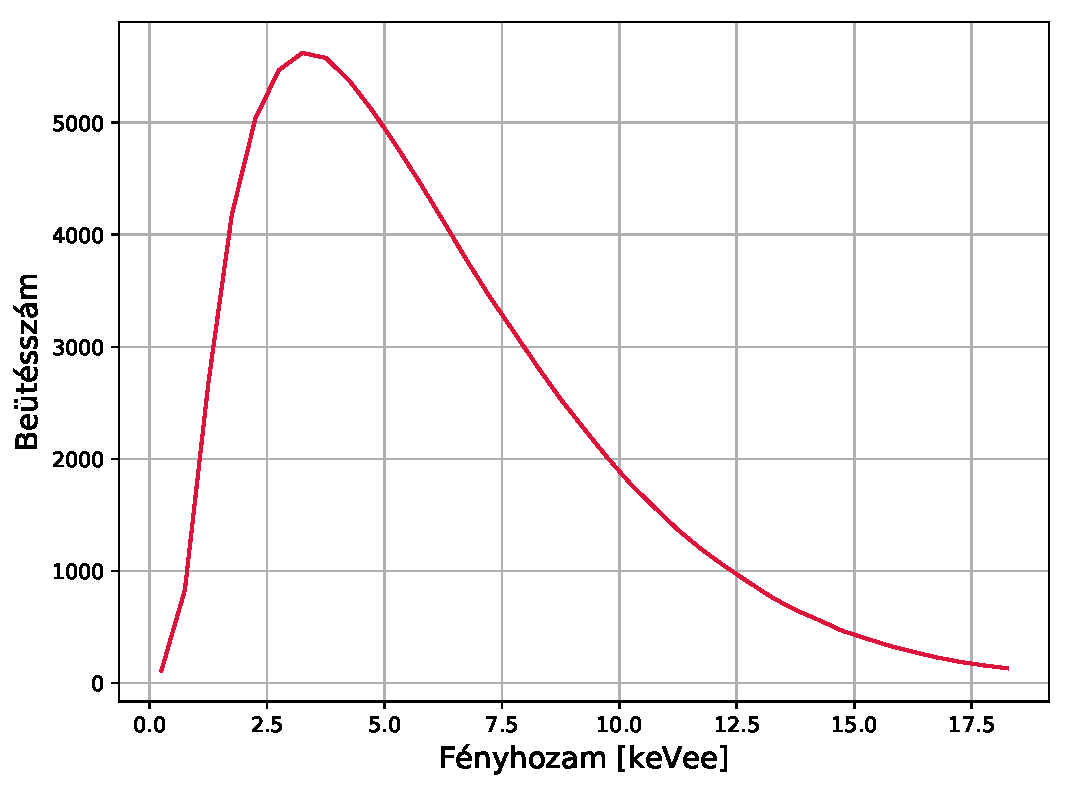
\includegraphics[width=0.8\linewidth ]{beta}
\caption{A mért spektrumok átlaga}
\end{figure}
\newpage
\hspace*{10pt} A másik módszerhez ki kell számolnunk a korábbi mérések átlagát, majd meg kell vizsgálnunk az új mérési sorok ettől vett eltérését. Amennyiben nincs szisztematikus eltérés, az esetben a két mérési sor a zaj erejéig ugyanazon mérésből származónak mondható, szisztematikus eltérés esetén azonban biztosan különbözik a két mérési sorozat.\\
\hspace*{10pt} A harmadik vizsgálati módszer a t-próba. Ennek során azt vizsgáljuk meg, hogy a két adatsort mekkora valószínűséggel állíthatta elő ugyanaz a folyamat.\\
\hspace*{10pt} Első lépésként megvizsgáltam mennyiben tér az új adatsorok átlaga a korábban felvett adatsor megfelelő értékétől. A számolások eredménye a \ref{fig:1a}. ábrán látható. A korábbi mérésből származó adatsorok átlaga $\overline{E}=5.931$ keV volt. Az ábrán látható, hogy az egyes későbbi mérésekből kapott átlagérték közel megegyezik ezzel, azonban kicsi szisztematikus eltérést mutat.\\
\begin{figure}[!h]
\centering
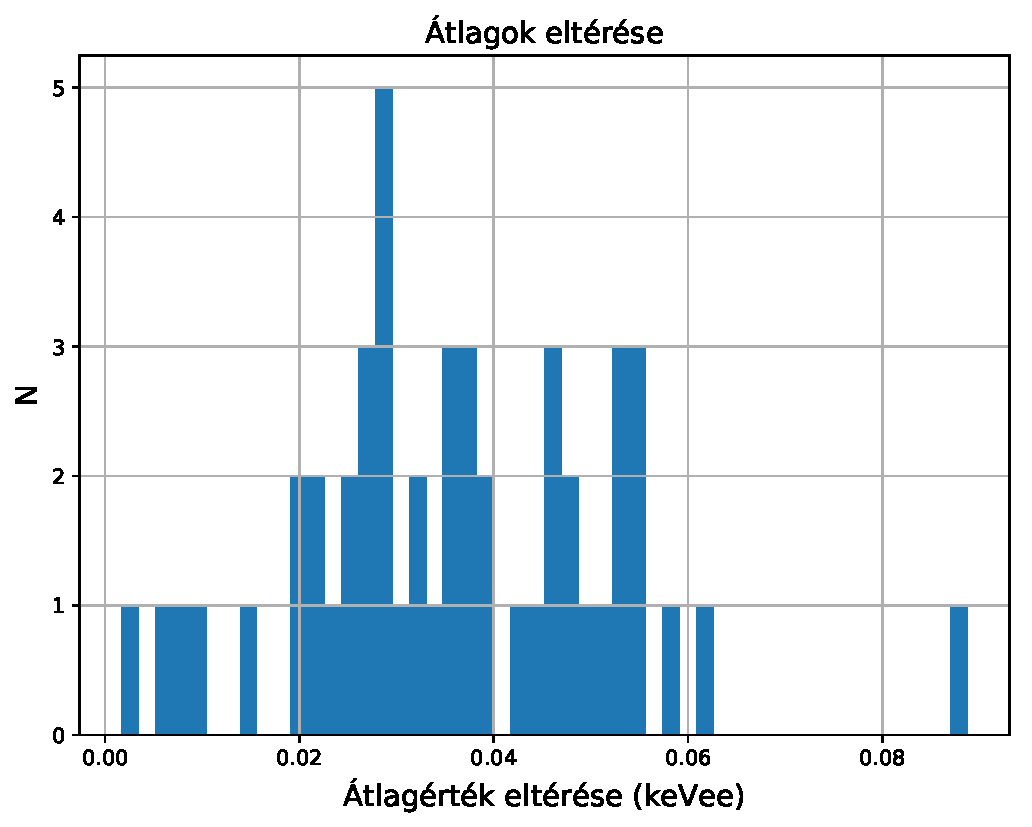
\includegraphics[width=0.8\linewidth]{atlag}
\caption{A későbbi méréssor átlagértékeinek és az összehasonlításhoz használt átlagérték eltérése hisztogram formájában ábrázolva.}
\label{fig:1a}
\end{figure}

\hspace*{10pt} Megvizsgáltam az egyes mért spektrumok korábbiaktól vett eltérését is. Ehhez kiszámoltam az átlagos spektrumot a korábbi adatsorokhoz, majd kivontam ezt az újabb adatsorokból. A kapott különbségnek képeztem az átlagát, mivel ha szisztematikus eltérés van, akkor annak fellelhetőnek kell lennie az átlagos spektrumokban is. A újonnan kapott spektrumokból kivontam a korábbi átlagspektrumot, ezzel kapva a \ref{fig:2a}. ábrát. Az ábrán jól látható, hogy a beütésszám becsült hibáján belül (melyet tisztán Poisson-hibának feltételeztem) az újonnan kapott spektrumok szisztematikus eltérést mutatnak, vagyis a beállítások megváltoztak a korábbi mérések óta, mindazonáltal az eltérések összemérhetők a becsült hibával.
\newpage
\begin{figure}[!h]
\centering
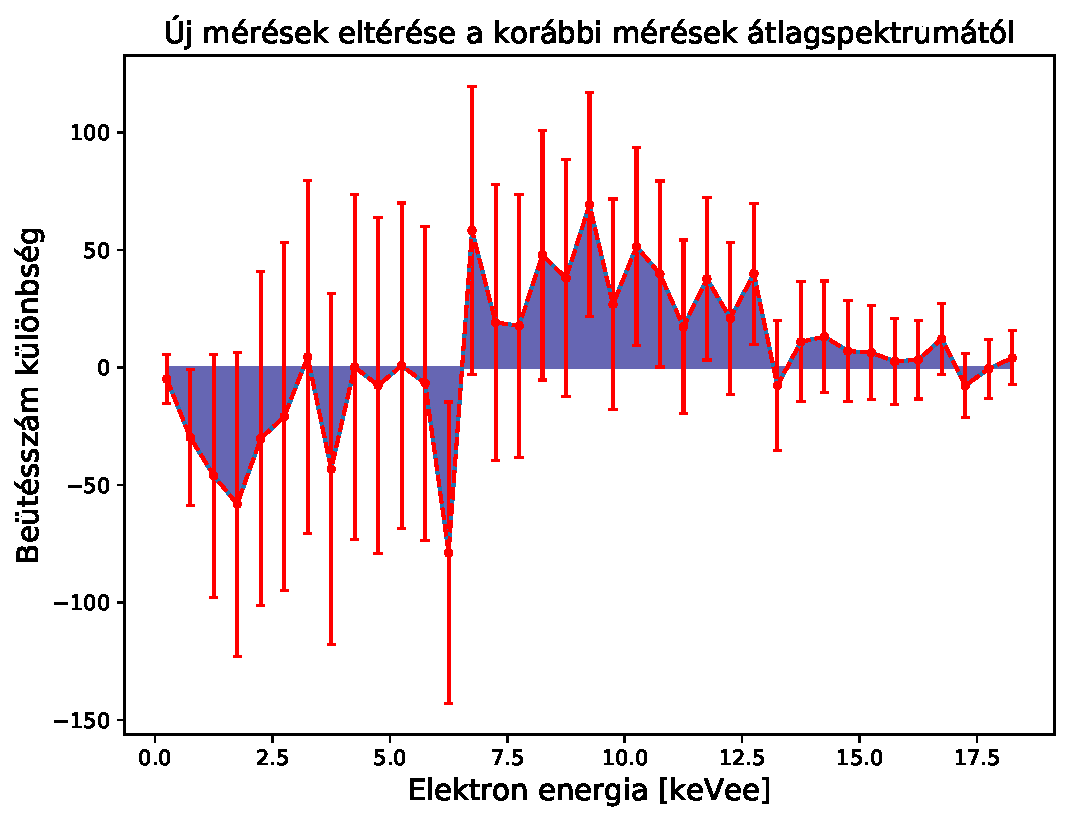
\includegraphics[width=0.8\linewidth]{elteres}
\caption{A későbbi méréssor és a későbbi mérések átlagos eltérése.}
\label{fig:2a}
\end{figure}
\hspace*{10pt} Az eddigi két vizsgálati módszerből tehát azt kaptuk, hogy bár bizonyos szisztematikus eltérés van a két adatsor között, de ez közel azonos nagyságrendű a becsült hibával. Harmadik vizsgálatként elvégeztem a t-próbát is a két adathalmazon, melyhez a python program \emph{scipy.stats.ttest\_ind} függvényét használtam. Ez egy olyan módszer, mely során azon null-hipotézist vizsgáljuk, hogy két független minta azonos átlaggal rendelkezik. A programnak a korábbi és az új méréssor átlagspektrumát adtam be, melyre kiszámolta, mekkora valószínűséggel származhat a két minta azonos eloszlásból. A futtatás után a valószínűségre p=0.99017-at kaptam, vagyis a két minta nagy valószínűséggel ugyanazon eloszlásból származott.\\
\hspace*{10pt} Összegezve a fentieket, a korábbi, illetve az újabb mérések között az erősítés mérési hibán belül nem változott, ugyanazok voltak a mérés paraméterei.

\subsection{A trícium spektrumok átlaga}
\hspace*{10pt} Következő feladatként az kellett megvizsgálnom, valóban visszakapjuk-e a mérésből az elméleti $\frac{1}{3}Q$ értéket. A számláshoz mind az ötven spektrum esetére kiszámoltam az átlagos fényhozam értékét, majd tekintettem ezek átlagát és szórását. A számolt értékeket az \ref{tab:atlagok}. táblázat tartalmazza.\\
\begin{table}
\begin{center}
\begin{tabular}{|c||c||c||c||c|}
\hline
$\overline{L}$ [keVee]& $\overline{L}$ [keVee]& $\overline{L}$ [keVee]& $\overline{L}$ [keVee]& $\overline{L}$ [keVee]\\
\hline
5.989 & 5.997 & 6.000 & 5.990 & 5.965\\
\hline 
6.016 & 5.987 & 6.009 & 5.999 & 5.971\\
\hline 
5.978 & 5.984 & 5.973 & 5.992 & 5.969\\ 
\hline 
5.993 & 5.992 & 6.009 & 5.996 & 6.022\\ 
\hline 
6.015 & 5.995 & 5.990 & 5.999 & 6.000\\ 
\hline 
5.984 & 5.993 & 5.983 & 6.019 & 5.983\\ 
\hline 
5.989 & 5.990 & 6.014 & 6.011 & 5.998\\ 
\hline 
6.006 & 6.007 & 6.018 & 6.002 & 6.016\\ 
\hline 
5.992 & 5.991 & 6.001 & 6.025 & 6.013\\ 
\hline 
6.011 & 6.009 & 6.018 & 6.000 & 6.052\\ 
\hline 
\end{tabular}
\caption{Az átlagos fényhozam értékek}
\label{tab:atlagok}
\end{center}
\end{table}
\hspace*{10pt} Az átlagos fényhozam érték 5.999 keVee volt. Eszerint a mérésből származó átlagos energia 0.2 keV-vel kisebb, mint amit a számítások alapján várnánk. Annak érdekében, hogy megvizsgáljuk, nem-e csak statisztikus hibáról van szó, kiszámoltam a kapott átlagértékek szórását is az empirikus szórás képletével:
\begin{equation}
\sigma=\sqrt{\frac{\sum_{i=1}^{N}(x_i-\overline{x})^2}{N-1}},
\end{equation}
ahol $N$ a mérések száma. A képlet használatával kapott szórás értéke: 
$$\sigma=0.016 \textrm{ keVee}.$$
A kapott érték segítségével kiszámolható, hogy a szórás hányszorosa a mérésből és a számolásból származó energiaérték különbsége:
\begin{equation}
\Delta=\frac{|<E>_{\textrm{számolt}}-<E>_{\textrm{mért}}|}{\sigma}=12.377
\end{equation}
Tehát a szórás több mint 12-szeresénél nagyobb a két érték különbsége, tehát szinte biztosan mondható, hogy a két érték különbsége nem statisztikus eredetű.\\
\hspace*{10pt} Az értékek különbségére magyarázatként szolgálhat a $quenching$ (eltolódás) jelensége, melynek köszönhetően kevesebb foton fog jutni a fotoelektron sokszorozóra, mivel a fotonok egy része el fog nyelődni a mintatartó üvegcse falában. Ennek eredményeképpen a teljes spektrum fel fog torlódni a kisebb energiák felé, így kisebb átlag fényhozamot, azaz kisebb átlagenergiát mérhetünk. $Quenching$-et több jelenség is okozhat, például a mintában, vagy a mintatartón található szennyeződések, melyek elnyelik a fotonokat.

\newpage
\subsection{Átlagspektrum szórása}
\hspace*{10pt} Mérésünk során áramimpulzusokat, azaz áttételesen beütéseket mértünk, melyek időben véletlenszerűen, egymástól függetlenül játszódtak le. Az ilyen események esetén tudjuk, hogy a beütésszámok hibáját Poisson-hibaként, azaz a beütésszám gyökeként írhatjuk le. Ezt az elméletet kellett leellenőriznem a kapott méréssorok alapját. Ehhez kiszámoltam az újabb mérések esetére az átlagspektrumot, majd minden csatorna, azaz  fényhozam érték esetére tekintettem az egyes spektrumok átlagtól való eltérését, vagyis kiszámítottam a szórást. Az elmélet vizsgálatához ábrázoltam a számolt szórást a csatornákban mérhető beütésszám függvényében, majd az elméletnek megfelelően hatványfüggvényt próbáltam illeszteni az adatokra. Az illesztés a \ref{fig:3}. ábrán látható.\\
\begin{figure}[!h]
\centering
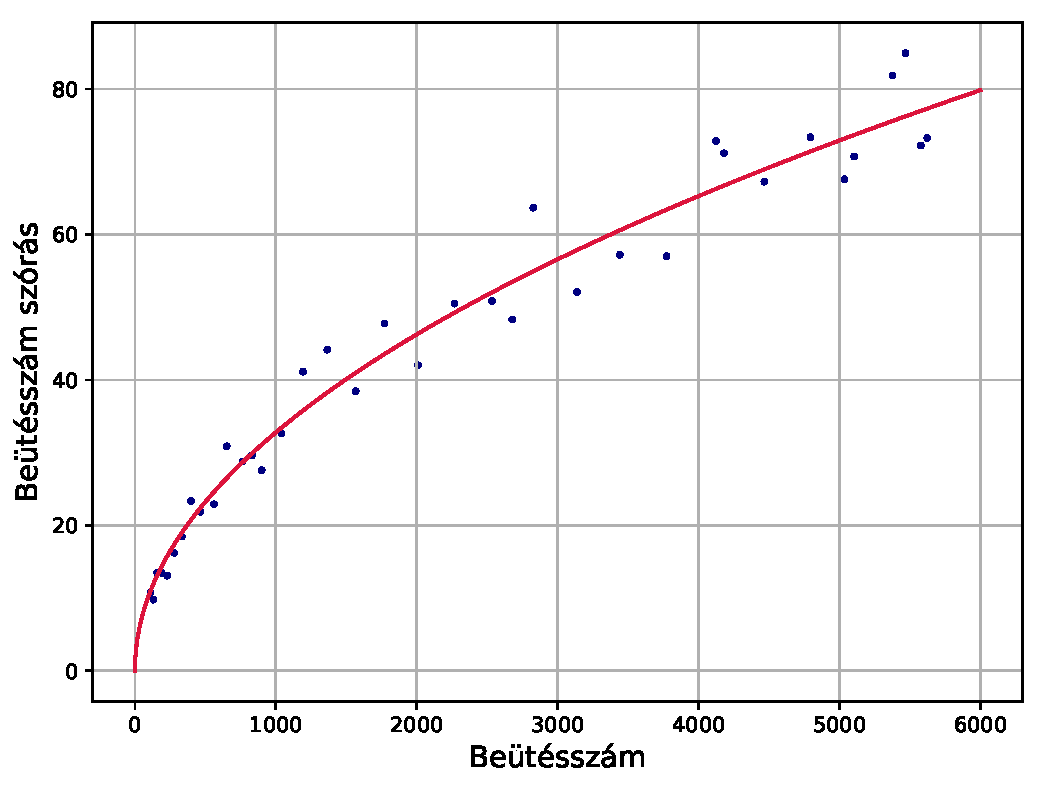
\includegraphics[width=0.8\linewidth]{poiss}
\caption{A számolt szórásértékekre történő illesztés}
\label{fig:3}
\end{figure}
\newline
\hspace*{10pt} Az illesztett görbe alakja:
$$ f(x)= (1.061 \pm 0.179) \cdot x ^{0.497 \pm 0.021}, $$
mely jó közelítéssel valóban négyzetgyök függvénynek felel meg.

\newpage
\section{Diszkusszió}
\hspace*{10pt} Mérésünk során megvizsgáltuk a trícium $\beta$ bomlását, megismerkedtünk a folyadékszcintillációs mérési módszerrel. A kapott spektrumok átlagenergiáját számolva az elméletihez közeli értéket kaptam, melyek közötti nem elhanyagolható eltérést az instrumentális eredetű csillapítással magyaráztam. Az átlagos spektrumtól történő eltérések vizsgálatával bizonyítottam a beütések hibájának Poisson-hibának megfelelő viselkedését is.

\section*{Hivatkozások}
\begin{itemize}
\item[(1).:] {http://metal.elte.hu/oktatas/alkfizlab/meresleirasok/FSS.pdf}

\end{itemize}
\end{document}
\end{document}